% "{'classe':('PSI'),'chapitre':'stat_pfs_2d','type':('application'),'titre':'Suspension automobile', 'source':'Florestan Mathurin','comp':('B2-14','C1-05','C2-07'),'corrige':True}"
%\setchapterimage{fig_00.jpg}
\chapter*{Application \arabic{cptApplication} \\ 
Suspension automobile -- \ifprof Corrigé \else Sujet \fi}
\addcontentsline{toc}{section}{Application \arabic{cptApplication} : Suspension automobile -- \ifprof Corrigé \else Sujet \fi}

\iflivret \stepcounter{cptApplication} \else
\ifprof  \stepcounter{cptApplication} \else \fi
\fi

\setcounter{question}{0}
\marginnote{Ressources de Florestan \textsc{Mathurin}.}
\marginnote[1cm]{
\UPSTIcompetence[2]{B2-14}
\UPSTIcompetence[2]{C1-05}
\UPSTIcompetence[2]{C2-07}
}







%
%\subsection*{Pilote automatique de voilier}
%\setcounter{exo}{0}
%\begin{center}
%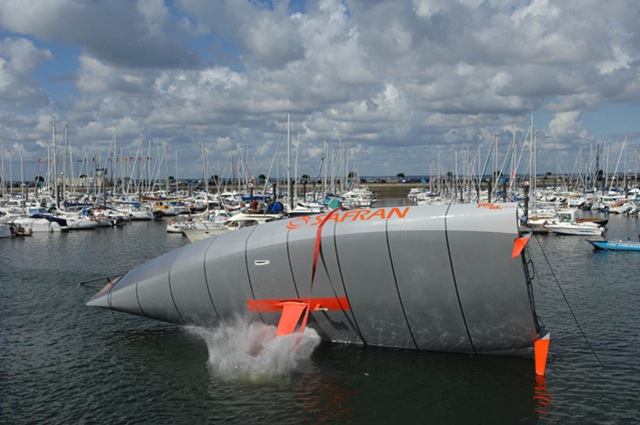
\includegraphics[width=.8\linewidth]{images/safran}
%
%\textit{Safrans... du SAFRAN (Skipper Marc Guillemot)}
%\end{center}
%
%\begin{center}
%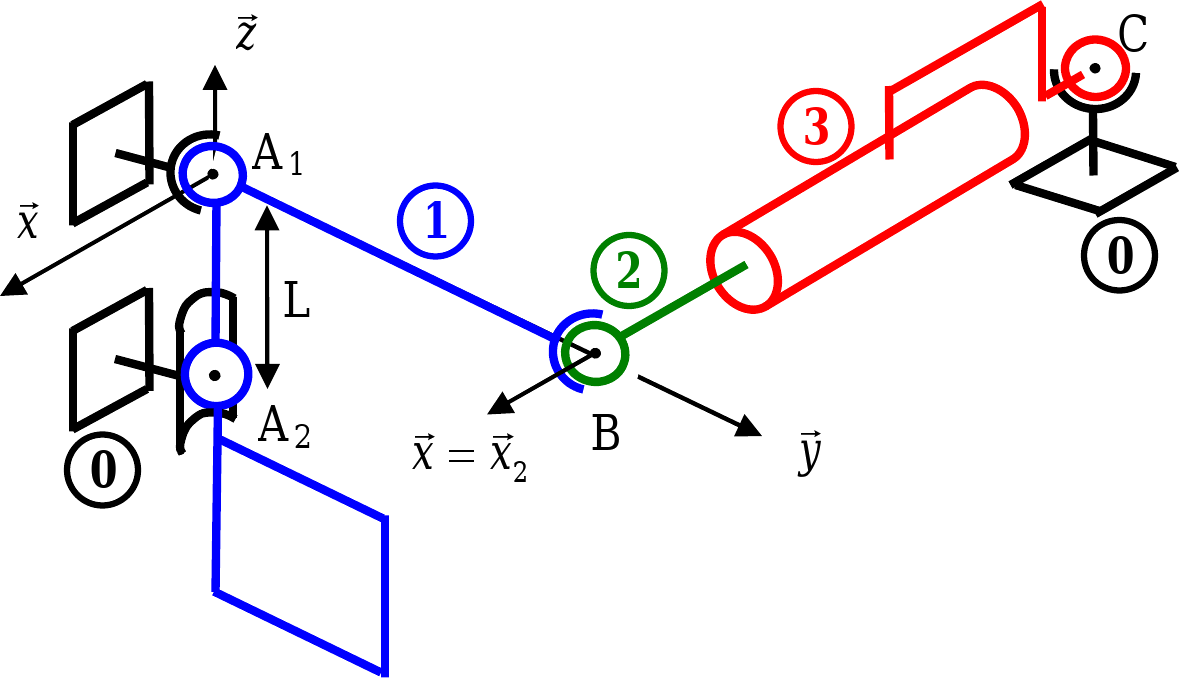
\includegraphics[width=\linewidth]{images/safran2}
%
%\textit{Schéma d'architecture}
%\end{center}
%
%
%
%
%Le safran d'un voilier lui permet de se diriger. Dans le cas du pilote hydraulique du laboratoire, l'angle du safran est asservi afin de pouvoir maintenir un cap, en tenant compte des aléas extérieurs (courants marins, vents violents...). Le safran est actionné par un vérin hydraulique, la pièce 2 étant relié à la tige du vérin et la pièce 3 constituant le corps du vérin. La pièce 1 représente le safran sur lequel agit la pression de l'eau $p$, perpendiculairement au plan du safran. 
%
%L'objectif de l'étude est de calculer les efforts dans les liaisons dans le but ultérieur de dimensionner le vérin hydraulique et les éléments mécaniques assurant les liaisons (éléments roulants ou coussinets). 
%
%
%
%%\begin{minipage}[c]{.6\linewidth}
%
%
%On donne : 
%\begin{itemize}
%\item $\vect{A_1B}=h\vect{y}$
%\item $\vect{CB}=\lambda\vect{x}$
%\end{itemize}
%
%\subparagraph{}
%\textit{Tracer le graphe de structure associé au système.}
%
%NB : il serait possible d'écrire la loi Entrée -- Sortie liant la vitesse de déploiement du vérin à la vitesse de rotation du safran.
%
%\subparagraph{}
%\textit{Sur le graphe d'architecture du système indiquer par des flèches les actions mécaniques agissant sur chacune des pièces.}
%
%Par la suite, on négligera l'action de la pesanteur sur les pièces 2 et 3. 
%
%%\end{minipage} \hfill
%%\begin{minipage}[c]{.35\linewidth}
%\begin{center}
%{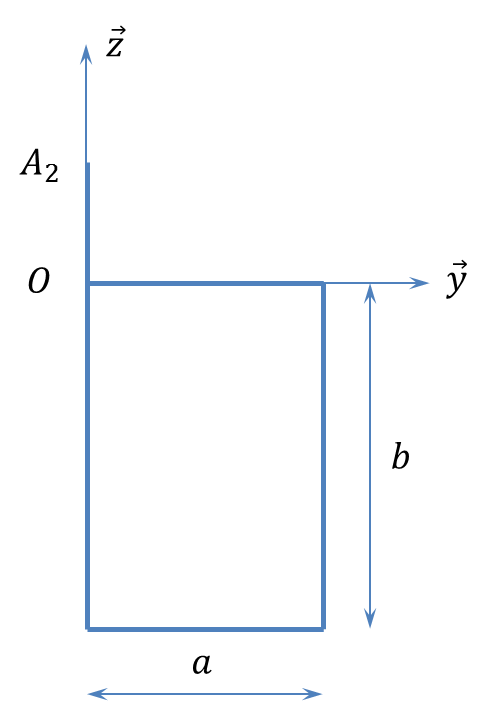
\includegraphics[width=.5\linewidth]{images/safran3}}
%\end{center}
%%\end{minipage}
%
%%\vspace{.5cm}
%
%\subparagraph{}
%\textit{Déterminer le torseur d'action mécanique de l'eau sur le gouvernail au point $A_2$. On considérera que $\vect{OA_2}=\vect{0}$. On négligera l'épaisseur du safran.} 
%
%%\subparagraph{}
%%\textit{Après avoir isolé le solide 1, appliquer le principe fondamental de la statique au point $A_1$.}
%%
%%\subparagraph{}
%%\textit{Quelles inconnues peuvent être déterminées ? Aurait-on pu le prévoir ?}
%%
%%\subparagraph{}
%%\textit{Après avoir isolé l'ensemble $\{2+3\}$, appliquer le principe fondamental de la statique au point $B$.}
%%
%%
%%\subparagraph{}
%%\textit{Quelles inconnues ont pu être déterminées ?}
%
%
%\subparagraph{}
%\textit{Déterminer l'effort à délivrer par le vérin pour supporter la pression de l'eau sur le safran.}
%
%\subparagraph{}
%\textit{Déterminer alors la pression à délivrer par le vérin en fonction d'une section $S$.}
%
%
%\subsection*{Bouche de climatisation}
%\setcounter{exo}{0}
%%\begin{minipage}[c]{.5\linewidth}
%On s’intéresse à une bouche de climatisation de bureau.   
%
%L’air climatisé arrive par le réseau d’air climatisé du bâtiment et est distribué par plusieurs bouches. Le débit d’air entrant sur chaque bouche est initialement réglé par l’intermédiaire d’un clapet dont l’ouverture est maîtrisée  par un vérin. On donne ci-dessous la modélisation sous forme de schéma d’architecture ainsi qu’un extrait de cahier des charges fonctionnel. 
%
%%\end{minipage} \hfill
%%\begin{minipage}[c]{.47\linewidth}
%\begin{center}
%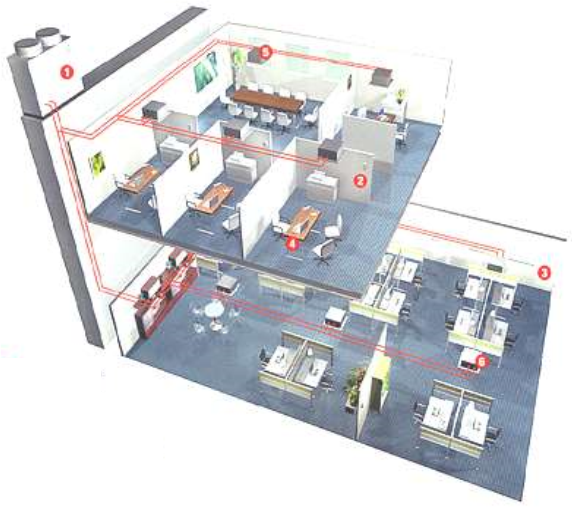
\includegraphics[width=.95\linewidth]{images/img1}
%\end{center}
%%\end{minipage}
%
%
%
%
%Le clapet 1, de masse $m$ et de centre de gravité $G (0,a,-h)$, est en liaison avec le mur 0 par l’intermédiaire d’une liaison rotule de centre $A (0,2a,0)$ et d’une liaison linéaire annulaire en $O$ d’axe $(O, \vect{y})$. Cette solution permet ainsi une rotation du clapet autour de l’axe $(O, \vect{y})$.
%
%L’air climatisé arrive par la bouche et exerce une poussée $\vectf{\text{air}}{1} = F_{\text{air}\rightarrow 1}\vect{x}$ en $M (0,a,-l)$.  
%
%Le débit d’air entrant est initialement réglé par l’intermédiaire de la raideur du vérin dont la tige est en liaison rotule et centre $B (0,2a+c,d)$  avec le clapet et en liaison rotule de centre $D (-e,2a+c,0)$  avec le mur 0. %La tige de vérin 2 exerce sur le solide 1 une poussée $\vectf{2}{1} = p.S \vect{x}$ 2 au point $B$.
%La résultante des actions de pression sur la tige 2 est notée $\vect{F_h}=pS \vect{x_2}$.
%%
%%\subparagraph{}
%%\textit{Donner la forme du torseur d’action mécanique transmissible de la liaison 0 sur 1 en $A$.}
%% 
%% \subparagraph{}
%% \textit{Donner la forme du torseur d’action mécanique transmissible de la liaison 0 sur 1 en $O$.}
%%
%% \subparagraph{}
%% \textit{Isoler l’ensemble 2+3 puis en déduire les expressions des torseurs d’action mécanique transmissible de la liaison 1 sur 2 en $B$ et de la liaison 0 sur 3 en $D$ que l’on écrira en projection dans la base 2 et 0.}
%% 
%  \subparagraph{}
% \textit{Déterminer la relation liant $p$ et 
% $\vectf{\text{air}}{1}$.}
% 
%\subparagraph{}
%\textit{On donne $S$ : section du piston du vérin. Déterminer la pression $p$ dans le vérin. Faire l’application numérique et conclure vis-à-vis du cahier des charges.}
%
%
%
%\ifprof
%\else
%\end{multicols}
%\fi
%
%\begin{center}
%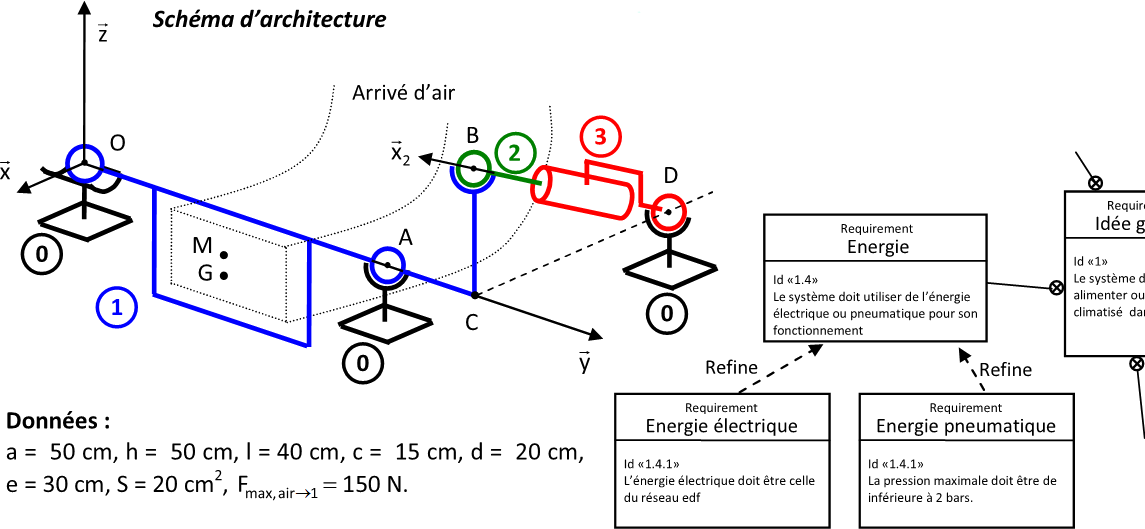
\includegraphics[width=.95\linewidth]{images/img2}
%\end{center}
%
%\newpage
%%\begin{center}
%%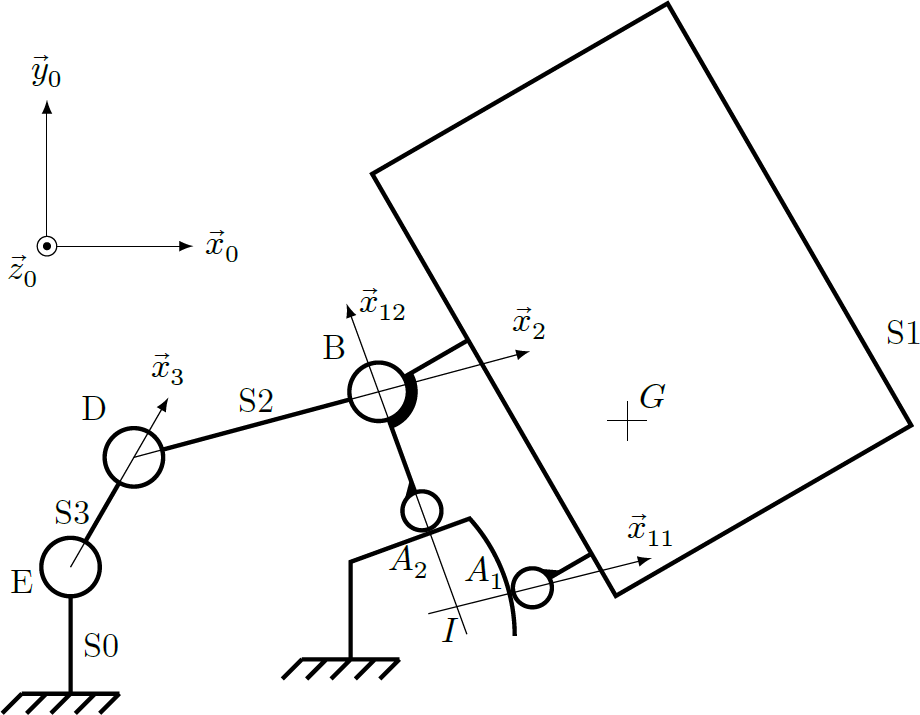
\includegraphics[width=\linewidth]{images/fig_04}
%%%\textit{}
%%\end{center}
%\begin{multicols}{2}

%\subsection*{Suspension automobile}
%\setcounter{exo}{0}


On s'intéresse à une suspension automobile dont on donne ci-dessous un extrait de cahier des charges fonctionnel ainsi qu’une modélisation. L'objectif est de vérifier si la suspension satisfait le niveau du critère d'affaissement statique maximal du cahier des charges, c'est à dire vérifier si la voiture, soumise à son propre poids, s'affaisse de moins ou de plus de 12 cm, suite à l'écrasement des amortisseurs. 


%
%
%\subparagraph{}
%\textit{Montrer que $Y_{43} =0$.}
%
%\subparagraph{}
%\textit{Déterminer les équations obtenues en appliquant le PFS à l’ensemble \{4+6\} au point $D$.}
%
%\subparagraph{}
%\textit{Montrer que $X_{92} =0$.}
%
%\subparagraph{}
%\textit{Déterminer les équations obtenues en appliquant le PFS au solide 2 au point $A$.}



\question{En minimisant le nombre d'équations, déterminer une relation entre $Y_{19}$ (action dans le ressort 9) et $F_{06}$.}

Données : $a = 16 \text{cm}$, $b = 33 \text{cm}$, $c = 8 \text{cm}$, $d = 25 \text{cm}$, $h = 3 \text{cm}$, $L = 15 \text{cm}$, $e = 9 \text{cm}$, $\mu = 18 \text{cm}$. 

La raideur du ressort est $k = 100\;000 \text{N/m}$. La masse de la voiture est de 2200 kg.

\question{Conclure quant à la capacité de la suspension de voiture à satisfaire l’exigence Affaissement statique du cahier des charges. }

\ifprof
\else
\begin{marginfigure}
\centering

\includegraphics[width=3cm]{Cy_11_Ch_03_PFS_2D_Application_02_FM_qr}
\end{marginfigure}
\fi

\begin{center}
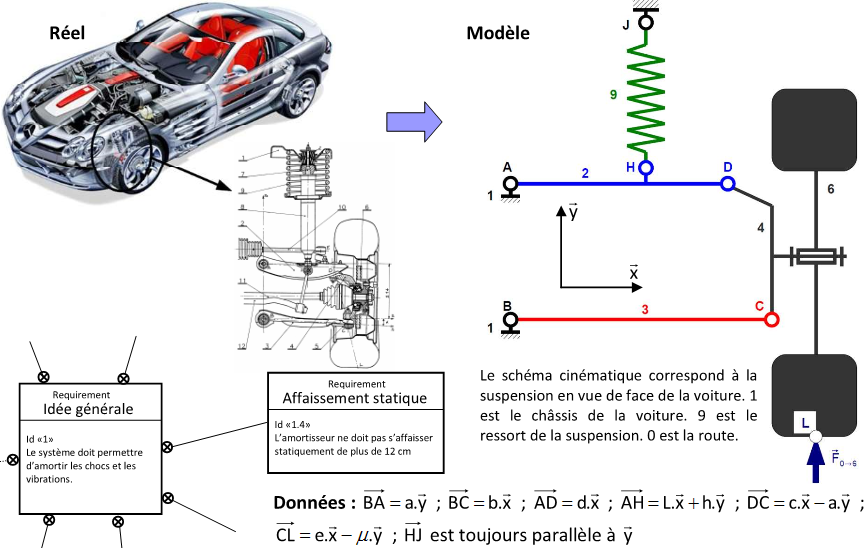
\includegraphics[width=\linewidth]{suspension}
\end{center}

